\section{概述}
\label{chap:analyze:overview}

%为什么要对丢包的特征进行检测
研究面向基于主动丢包的VoLTE时间隐通道的检测方法,对改进时间隐通道构建方法,提高抗检测能力有正向促进意义。VoLTE中音频信道存在明显的传输特征,传输过程中的丢包事件非常少,现有的时间隐通道检测方法,能够检测出异常传输现象。对于VoLTE视频信道,尤其是采用基于主动丢包的时间隐通道,时间隐通道对IPD分布产生的影响有限。传统的时间隐通道检测方法,无法完全反映丢包特征,检测效果较差。因此,针对该类时间隐通道,需要设计一种综合、高效的检测方法,从而提升检测水平及隐通道构建水平。

\insertFigure{
	\begin{figure}
		\centering
        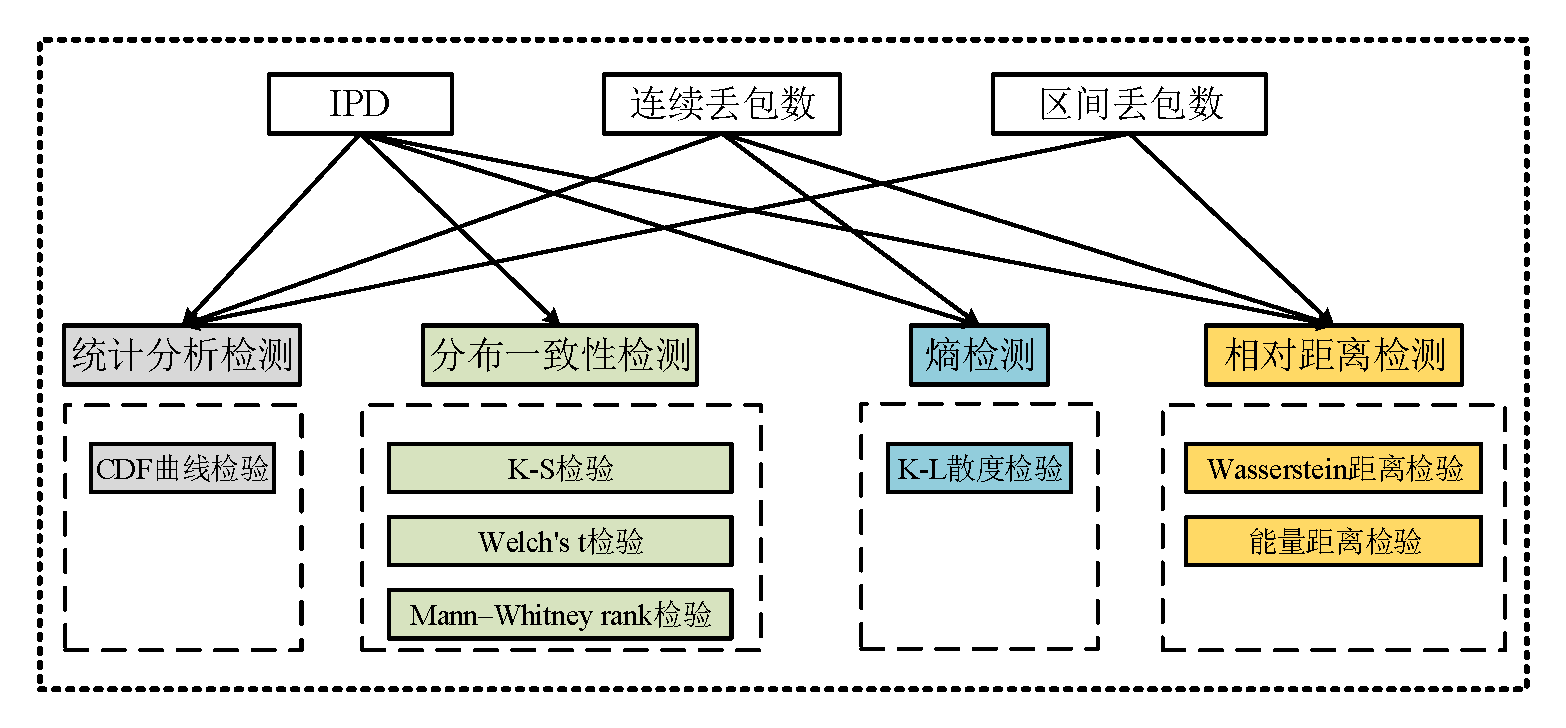
\includegraphics[width=0.9\textwidth]{chapters/chapter3/figures/struct.pdf}
        \caption{面向基于主动丢包的VoLTE时间隐通道检测方法结构图}\label{fig:3:struct}
	\end{figure}
}

%检测主要从IPD、丢包特征及突发丢包几个方面展开
丢包事件发生后,产生的影响体现在IPD分布、突发丢包长度及区间丢包数分布各方面。本检测方法的基础,是分析各统计特征在构建时间隐通道前后的差异。如图\nref{fig:3:struct},本检测方法的检测对象包括IPD、突发丢包长度及区间丢包数三种。采用的检测方法分为四类,分别为统计分析检测、分布一致性检测、熵检测及相对距离检测。基于IPD的检测方法,是时间隐通道的基本检测方法,IPD作为观测量,所有检测方法都对其适用。突发丢包长度的检测,重点在于判断不同长度突发丢包的概率,因此适用统计分析检测、熵检测及相对距离检测。区间丢包数的检测,重点在于判断分布之间的差异,因此适用统计分析检测及相对距离检测。
%通过模拟测试,该评估方法具备可行性
为检测该方法的可用性,设计了模拟主动丢包的时间隐通道进行测试。通过一系列模拟实验,证明了该方法综合了各维度特征后,提升了检测能力,对基于主动丢包的时间隐通道具有良好的分辨能力。